\chapter{Anexo B} 	
\begin{landscape}
\label{appendix-b}

\begin{figure}[H]
    \centering
    \subfloat[\centering Estado Inicial]{{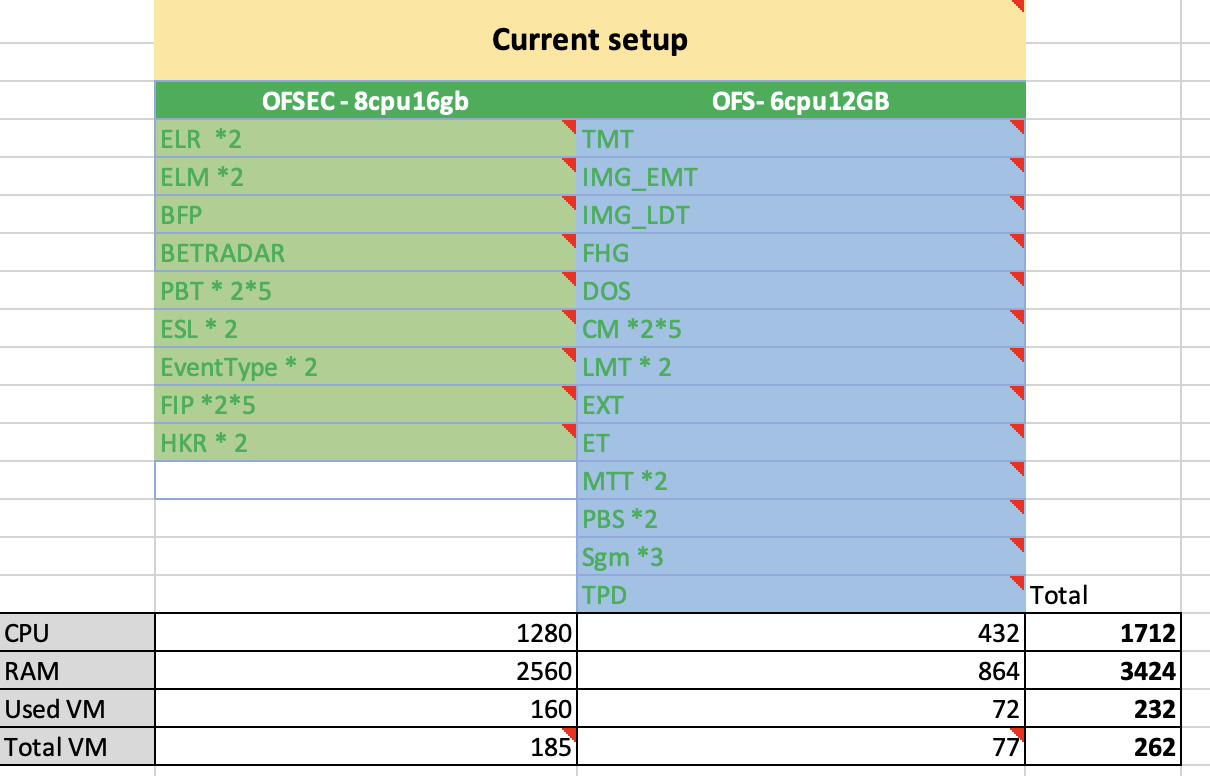
\includegraphics[width=0.6\textwidth]{media/content/analise/strat-current} }}%
    \qquad
    \subfloat[\centering Passo 1]{{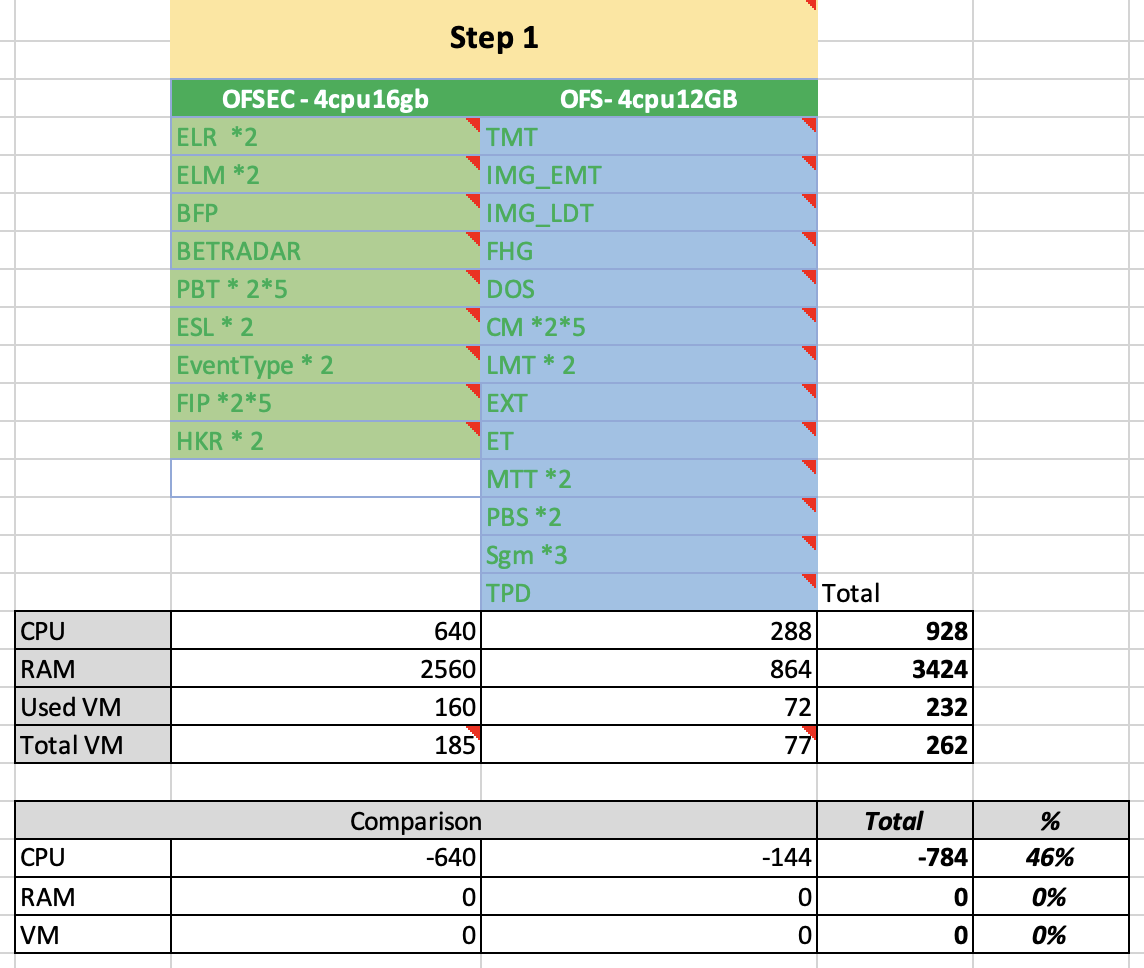
\includegraphics[width=0.6\textwidth]{media/content/analise/strat-1} }}%
    \caption{Comparação entre Estado Inicial e o Passo 1 da Implementação da Solução}%
\end{figure}

\begin{figure}[H]
    \centering
    \subfloat[\centering Passo 1]{{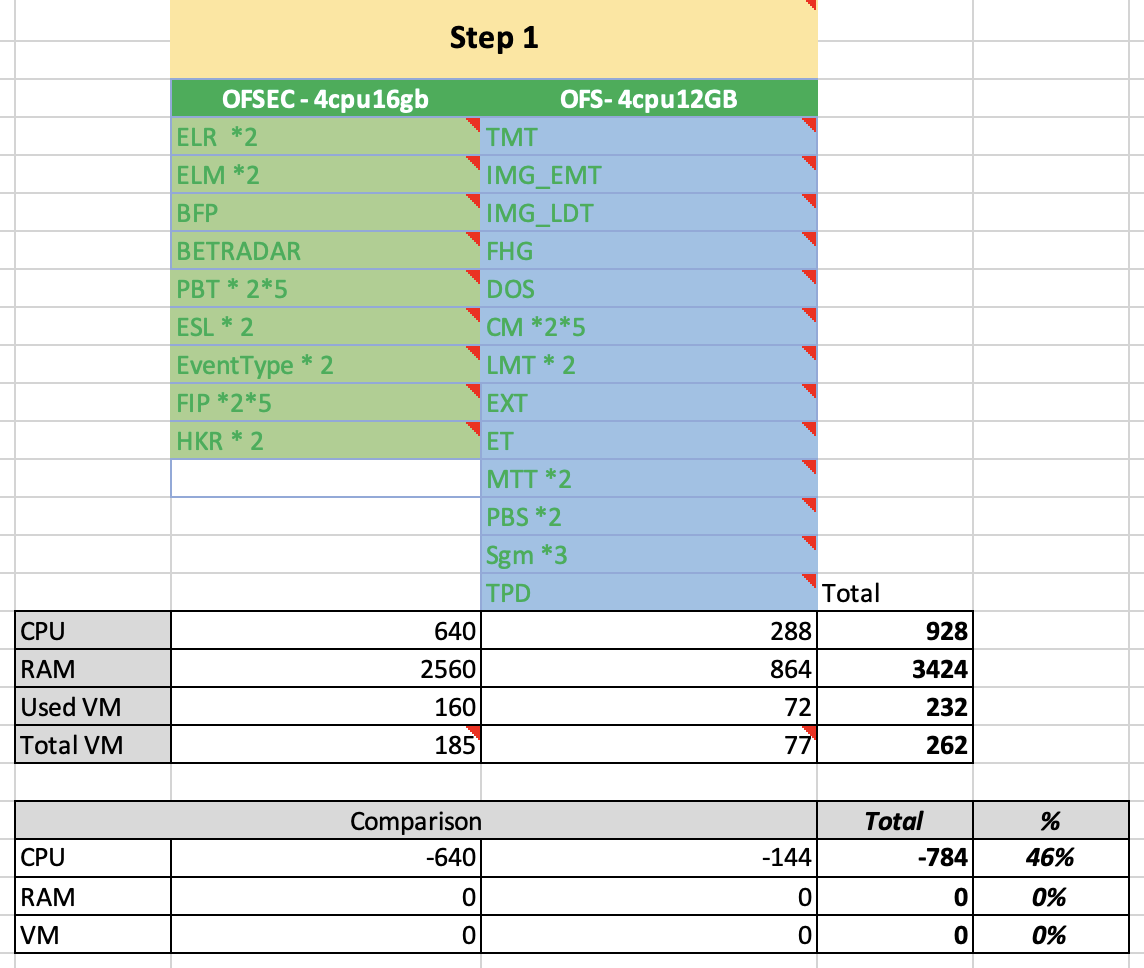
\includegraphics[width=0.6\textwidth]{media/content/analise/strat-1} }}%
    \qquad
    \subfloat[\centering Passo 2]{{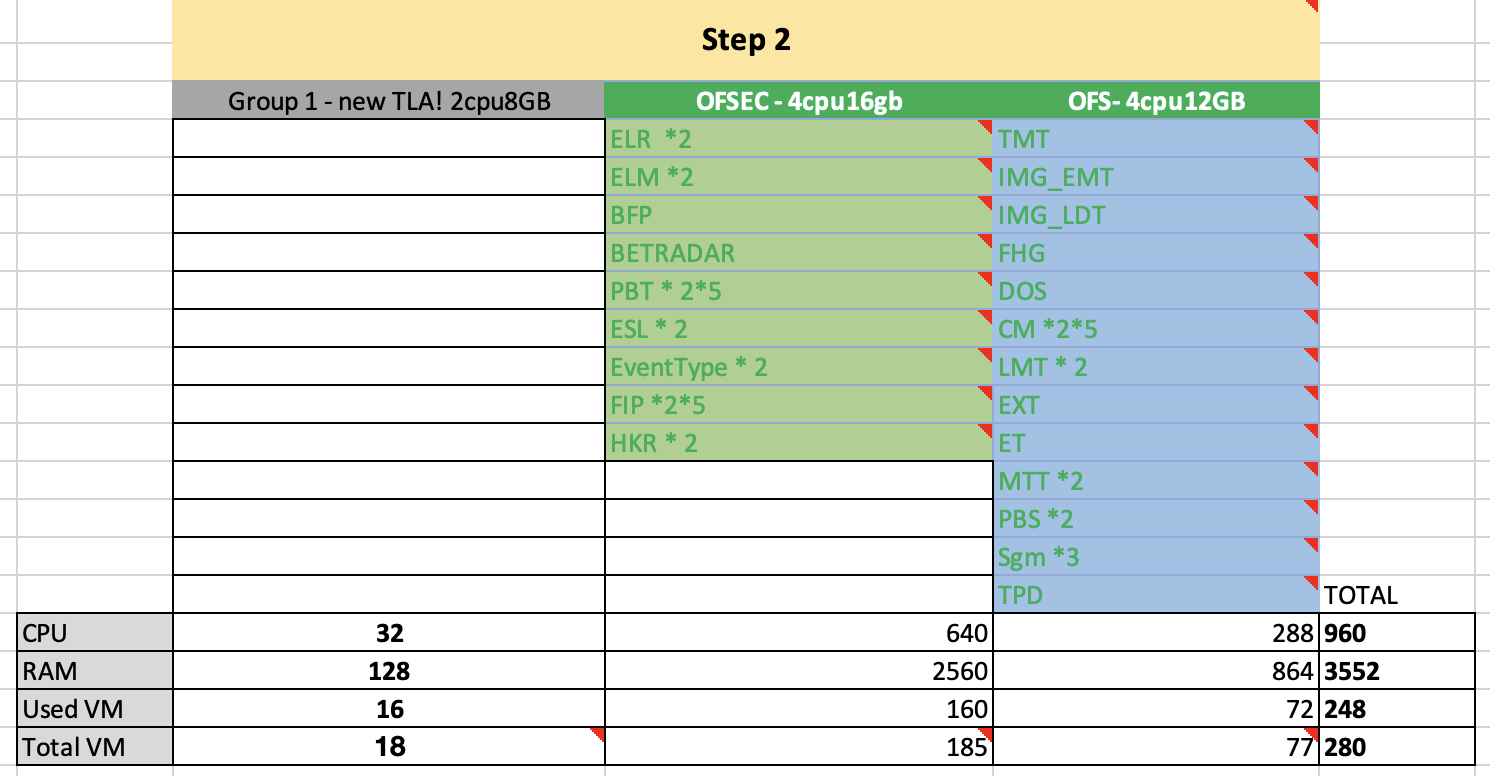
\includegraphics[width=0.6\textwidth]{media/content/analise/strat-2} }}%
    \caption{Comparação entre Passo 1 e o Passo 2 da Implementação da Solução}%
\end{figure}

\begin{figure}[H]
    \centering
    \subfloat[\centering Passo 2]{{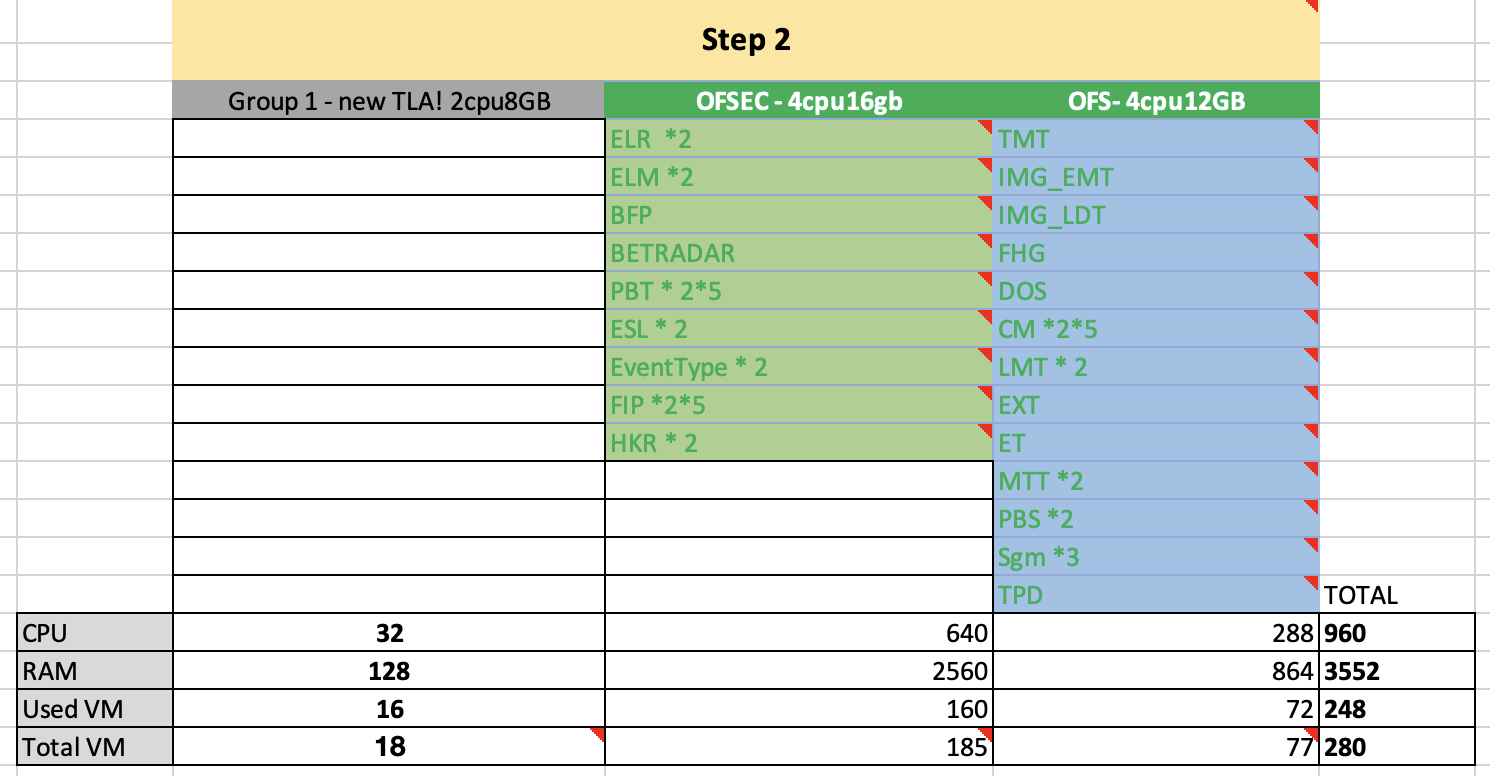
\includegraphics[width=0.6\textwidth]{media/content/analise/strat-2} }}%
    \qquad
    \subfloat[\centering Passo 2.1]{{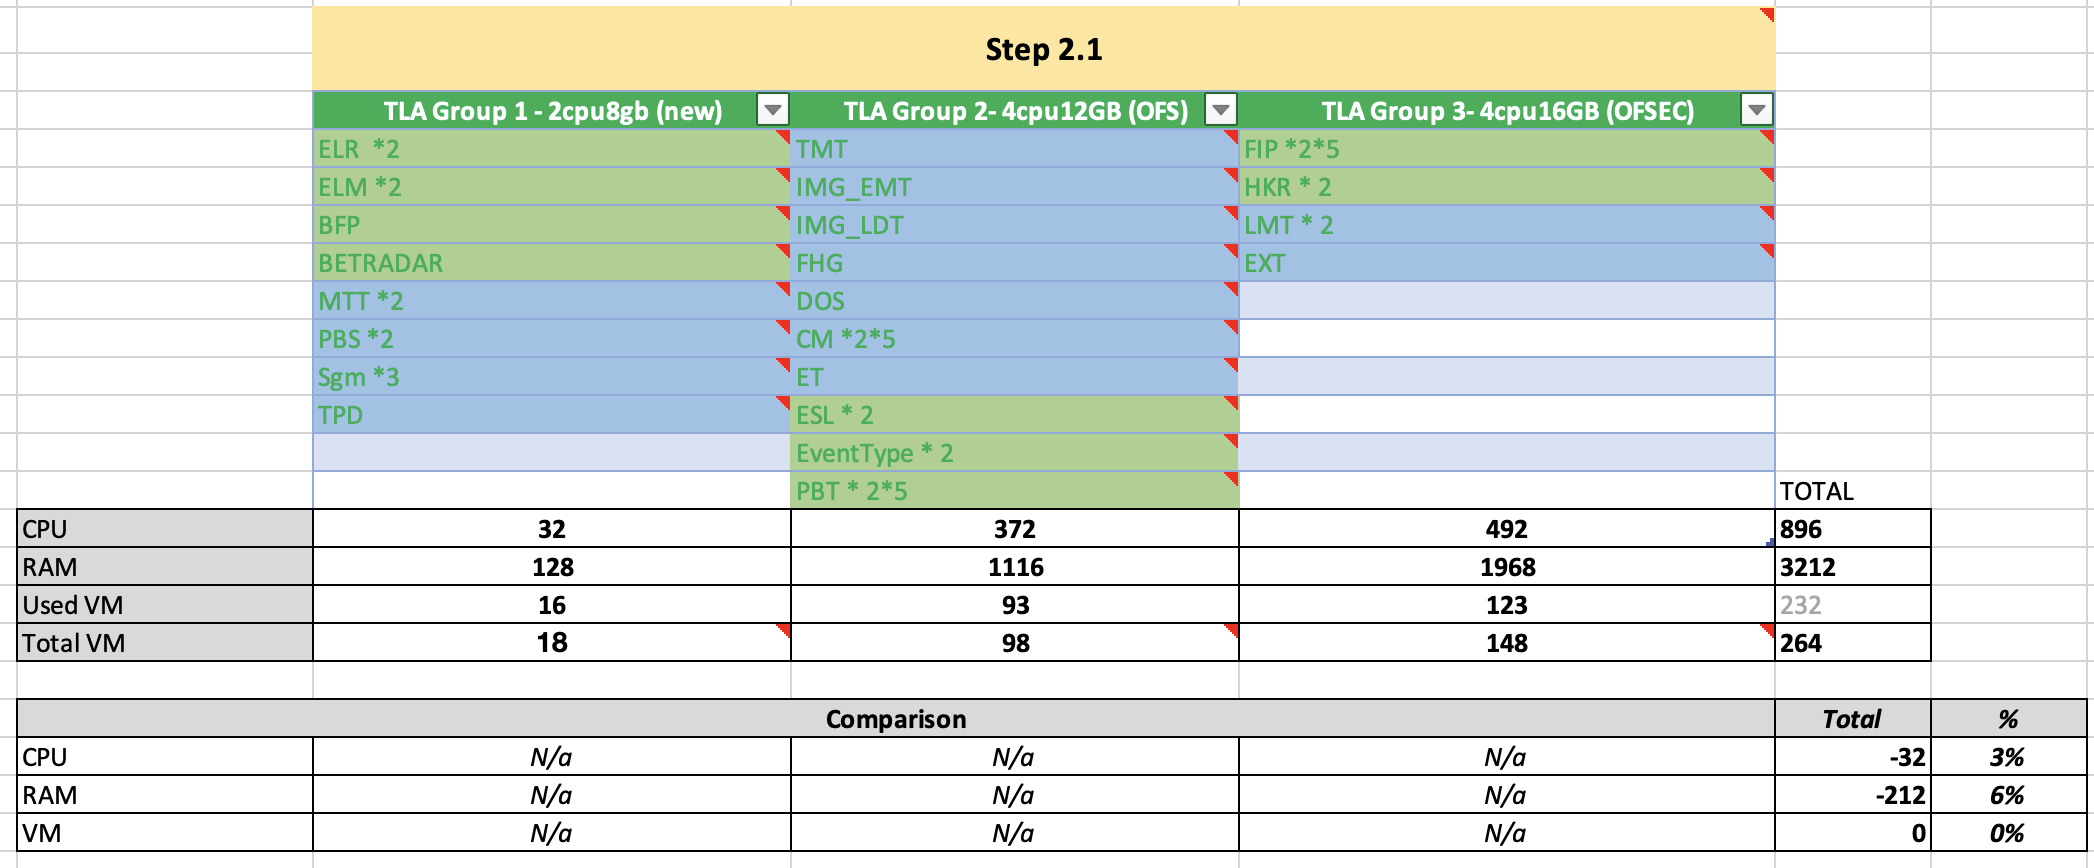
\includegraphics[width=0.6\textwidth]{media/content/analise/strat-2_1} }}%
    \caption{Comparação entre Passo 2 e o Passo 2.1 da Implementação da Solução}%
\end{figure}

\begin{figure}[H]
    \centering
    \subfloat[\centering Passo 2.1]{{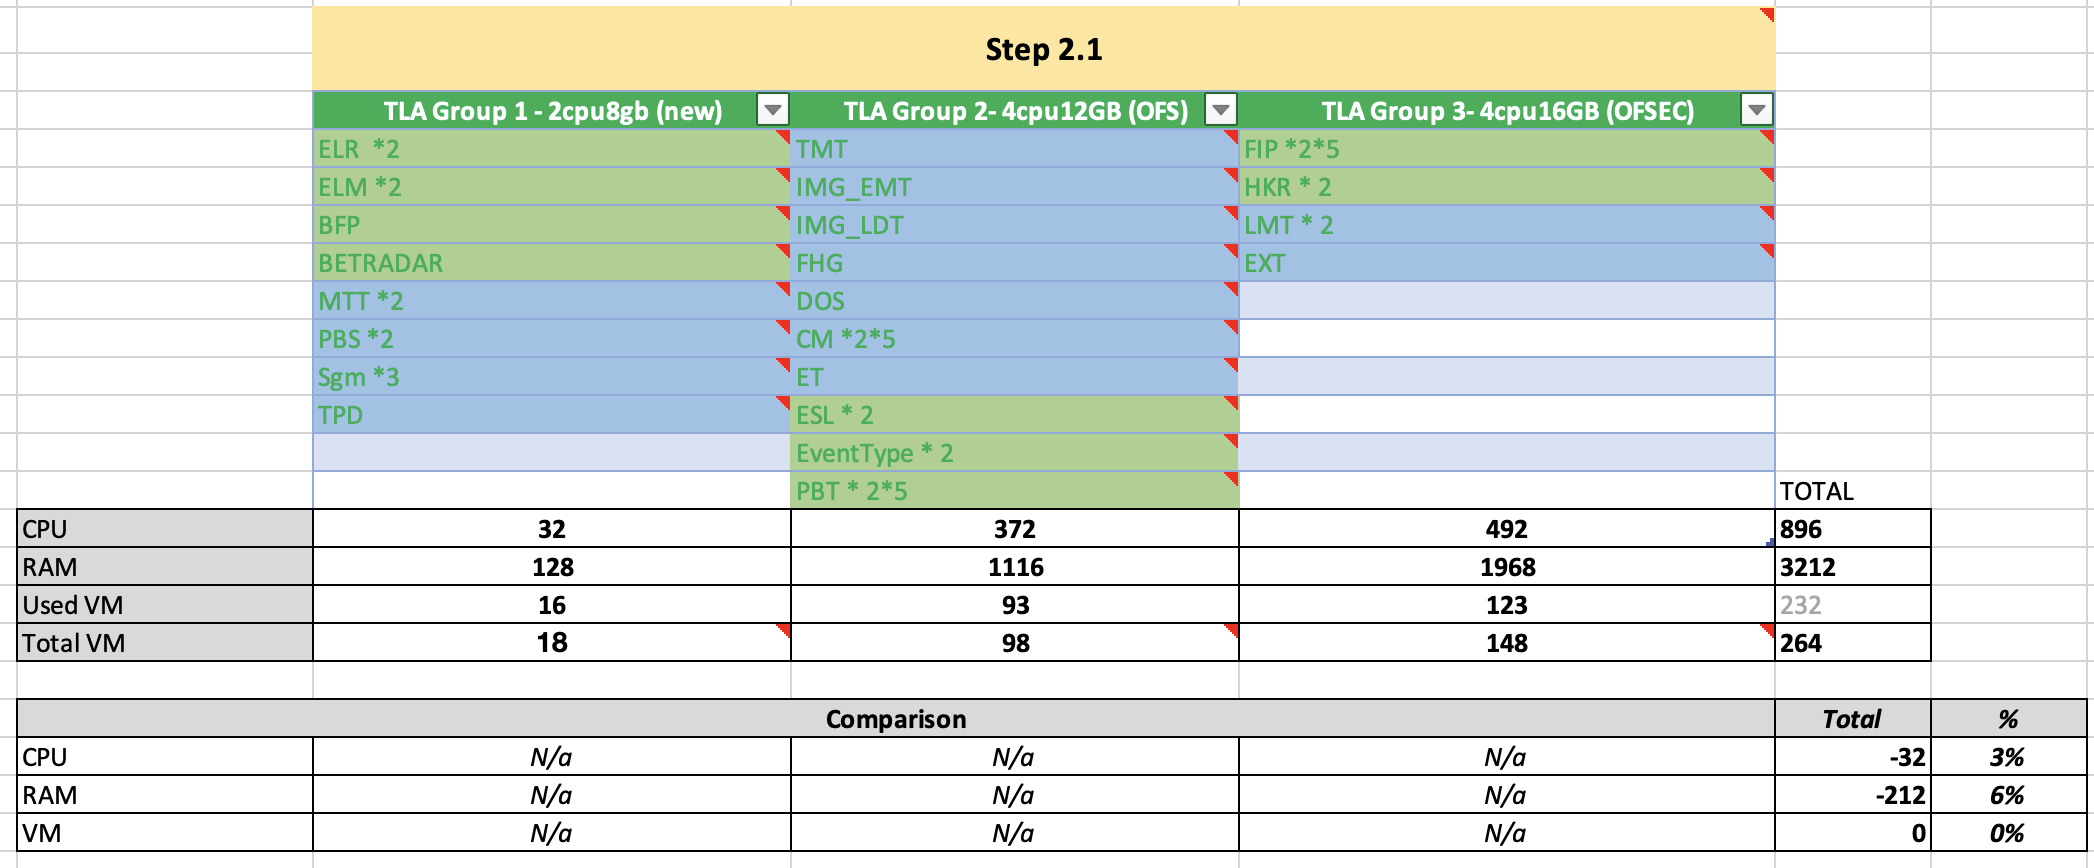
\includegraphics[width=0.6\textwidth]{media/content/analise/strat-2_1} }}%
    \qquad
    \subfloat[\centering Passo 2]{{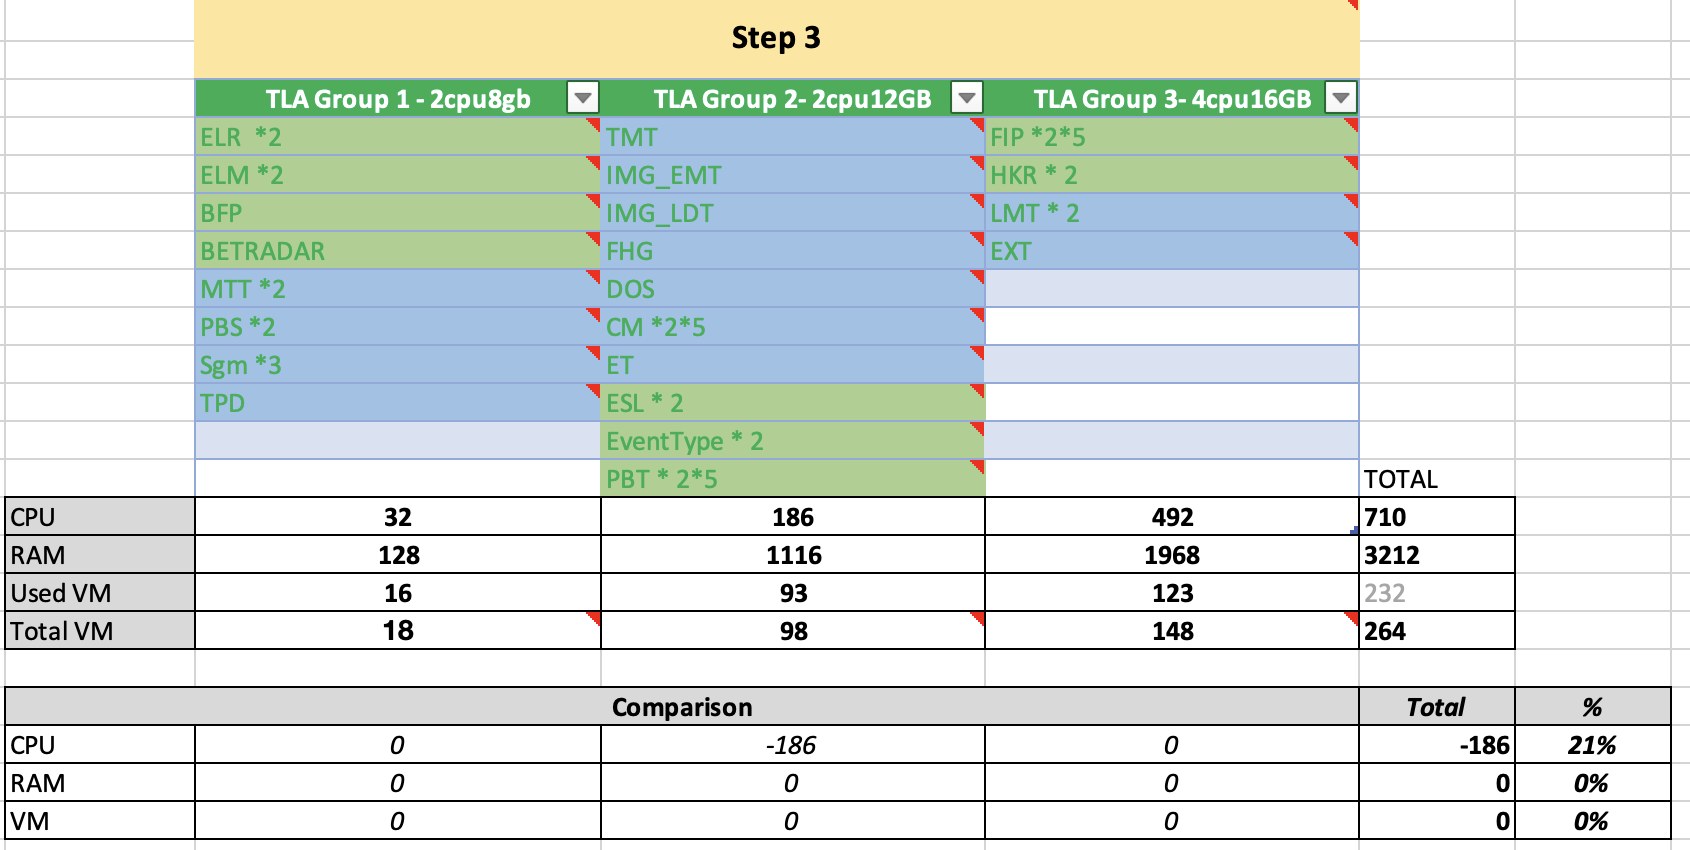
\includegraphics[width=0.6\textwidth]{media/content/analise/strat-3} }}%
    \caption{Comparação entre Passo 2.1 e o Passo 3 da Implementação da Solução}%
\end{figure}

\end{landscape}
